\documentclass{article}

\usepackage{geometry}
\usepackage{amsfonts, amsmath, amssymb, amsthm}
\usepackage{enumitem}
\usepackage{commands}
\usepackage{mathtools}
\usepackage{hyperref}
\usepackage{tikz}
\hypersetup{colorlinks, linkcolor={blue}, citecolor={blue}, urlcolor={blue}}

\newcommand{\dol}{\overline{\partial}}
\newcommand{\Cech}{\v{C}ech}
\newcommand{\cC}{\check{\mathcal{C}}}
\newcommand{\cH}{\check{\mathrm{H}}}

\begin{document}
\puttitle{What is Dolbeault cohomology}\self

\section{Preliminaries on complex manifolds}

A \emph{complex structure} $J$ on a real vector space $V$ is a linear map $J: V \to V$ such that $J^2 = -\id_V$. It equivalently provides a $\C$-vector space structure on $V$, so after complexification, we have a natural splitting
\[
    V \otimes_\R \C \simeq V_J \oplus \overline{V_J}
\]
into the two eigenspaces of $J\otimes \C$ with eigenvalues $\pm i$. 

An \emph{almost complex manifold} is a smooth manifold $M$ with a complex structure $J$ on the real tangent bundle $T$. The above discussion yields a splitting of complex vector bundles
\[
    T^*_{1,0}:=T^*,\quad T^*_{0,1}:=\overline{T^*},\quad T^* \otimes_\R \C \simeq T^*_{1,0} \oplus T^*_{0,1}.
\]
Since the exterior algebra functor $\Lambda^\bullet$ commutes with base change and colimits, we have
\[
    \Omega^i\otimes\C \simeq \Lambda^{i}(T^*\otimes\C) \simeq \bigoplus_{p+q=i} \Lambda^p(T^*_{1,0}) \otimes_\C \Lambda^q(T^*_{0,1}).
\]
To ease notation, denote the sheaves of $(p,q)$-forms by $\Omega^{p,q}\leftrightarrow \Lambda^p(T^*_{1,0}) \otimes \Lambda^q(T^*_{0,1})$. The (complexified) differential $d$ then decomposes as
\[
    d = \partial + \dol,
\]
where
\[
    \partial: \Omega^{p,q} \to \Omega^{p+1,q},\quad \dol: \Omega^{p,q} \to \Omega^{p,q+1}.
\]
These clearly satisfy $\partial^2 = 0$ and $\dol^2 = 0$, and hence also $\partial\dol+\dol\partial=0$.

In summary, the complexification of the de Rham complex $(\Omega^\bullet,d)$ results in a bigraded complex $(\Omega^{\bullet,\bullet},\partial,\dol)$.

\begin{definition}
    The \emph{Dolbeault complex} is the complex $(\Omega^{p,\bullet},\dol)$. The cohomology of the complex of its global sections is called the \emph{Dolbeault cohomology} and denoted by $H^{p,q}(M)$.
\end{definition}

So for example, if $p=0$, the Dolbeault complex is
\[
    0 \longrightarrow \Omega^{0,0} \xrightarrow{\ \dol\ } \Omega^{0,1} \xrightarrow{\ \dol\ } \Omega^{0,2} \longrightarrow \cdots
\]
and for higher $p$, the Dolbeault complex is obtained by tensoring the above with $\Omega^{p,0}$.

\begin{definition}
    A \emph{complex manifold} $(M,\mathcal{O})$ is a smooth manifold $(M,\mathcal{A})$ with a sheaf of holomorphic functions $\mathcal{O}\subset\mathcal{A}\otimes\C$, such that $\mathcal{O}$ is locally isomorphic to the sheaf of holomorphic functions on open subsets of $\C^n$.
\end{definition}

In this case, $T_{1,0}\simeq T$, as a $\C$-vector bundle, has a natural holomorphic structure. Hence it is sometimes called the \emph{holomorphic tangent bundle}.

Finally, consider the following analogue of the de Rham complex
\begin{equation}\label{eq:dol}
    0 \longrightarrow \mathcal{O} \longrightarrow \mathcal{A}\otimes\C \xrightarrow{\ \dol\ } \Omega^{0,1} \xrightarrow{\ \dol\ } \Omega^{0,2} \longrightarrow \cdots
\end{equation}
All the sheaves $\Omega^{\bullet,\bullet}$ are soft as $\mathcal{A}$-modules. To compute the cohomology, we have 

\begin{theorem}\label{thm.poin}
    \eqref{eq:dol} is exact, so the Dolbeault complex is a soft resolution of $\mathcal{O}$.
\end{theorem}

We defer the proof of this to the next section. 

\begin{corollary}
    Given any holomorphic vector bundle $E$, the following sequence is a soft resolution for the corresponding locally free $\mathcal{O}$-module $\mathcal{E}$.
    \[
        0 \longrightarrow \mathcal{E} \longrightarrow (\mathcal{A}\otimes\C)\otimes\mathcal{E} \xrightarrow{\ \dol\ } \Omega^{0,1}\otimes\mathcal{E} \xrightarrow{\ \dol\ } \, \cdots\, \xrightarrow{\ \dol\ } \Omega^{0,n}\otimes\mathcal{E} \longrightarrow 0
    \]
\end{corollary}

\begin{proof}
    Since $\dol$ is $\mathcal{O}$-linear, we apply $-\otimes_{\mathcal{O}}\mathcal{E}$ to \eqref{eq:dol}.
\end{proof}

Define $\mathcal{E}':=(\mathcal{A}\otimes\C)\otimes_{\mathcal{O}}\mathcal{E}$ if we wish to consider the sheaf of smooth sections instead. Any toddler will know how to rewrite the above resolution as
\[
    0 \longrightarrow \mathcal{E} \longrightarrow \mathcal{E}' \xrightarrow{\ \dol\ } \Omega^{0,1}\otimes\mathcal{E}' \xrightarrow{\ \dol\ } \, \cdots\, \xrightarrow{\ \dol\ } \Omega^{0,n}\otimes\mathcal{E}' \longrightarrow 0
\]
where $\otimes=\otimes_{\mathcal{A}\otimes\C}$. In particular, we've explained previously that the vector bundles corresponding to $\Omega^{p,0}$ are in fact holomorphic vector bundles. We quickly deduce that
\[
    0 \longrightarrow \mathcal{H}^p \longrightarrow \Omega^{p,0} \xrightarrow{\ \dol\ } \Omega^{p,1} \xrightarrow{\ \dol\ } \, \cdots\, \xrightarrow{\ \dol\ } \Omega^{p,n} \longrightarrow 0
\]
is a soft resolution for $\mathcal{H}^p$, the sheaf of holomorphic $p$-forms. Therefore

\begin{corollary}
    The Dolbeault cohomology with coefficients in a holomorphic vector bundle $E$ satisfies
    \[
        H^{p,q}(M,E) \simeq H^q(M,\mathcal{E}\otimes\mathcal{H}^p).
    \]
    In particular, $H^{p,q}(M) \simeq H^q(M,\mathcal{H}^p)$, and so $H^{0,q}(M) \simeq H^q(M,\mathcal{O})$.
\end{corollary}

\section{Dolbeault-Grothendieck Lemma}

In the results of this section, we will take smooth sections defined globally on some affine space $\C^n$ and discuss their properties over a certain open subset $V$. However, it clearly suffices to define these functions on any neighborhood of $\overline{V}$.

\begin{lemma}\label{lem.cauchy}
    If $V$ is a bounded open subset of $\C$ and $f\in\mathcal{A}\otimes\C(\C)$ is compactly supported, then there exists $g\in\mathcal{A}\otimes\C(\C)$ such that $\dfrac{\partial}{\partial\overline{z}}g=f$ on $V$. One such $g$ is given by the formula
    \[
        g(a) := \frac{1}{2\pi i} \int_{V} \frac{f(z)}{z-a} dz\wedge d\overline{z},\quad \forall a\in\C.
    \]
\end{lemma}

\begin{proof}
    First, let's check that this integral makes sense. For small $\epsilon>0$, put $W=B_\epsilon(a)$. Since $dz\wedge d\overline{z}=-2i d\lambda=-2i\rho d\rho\wedge d\theta$, where $\lambda$ is the usual Lebesgue measure, we have
    \begin{align*}
        \int_{W} \abs{\frac{f(z)}{z-a}} d\lambda 
        = \int_{[0,2\pi]\times[0,\varepsilon]} \abs{\frac{f(a+\rho e^{i\theta})}{\rho e^{i\theta}}} \rho d\rho d\theta 
        = \int \abs{f(a+\rho e^{i\theta})} d\rho d\theta
        < \infty,
    \end{align*}
    where the first equality is the change of variable formula for non-negative functions, cf. \emph{Folland, Theorem 2.47}. Away from $W$, the integrand is smooth. This shows that $g$ is well defined. 
    
    If the singularity at $a$ is in $V$, one way to deal with it is the following trick. Take a smooth function $\mu$ such that $\mu(W)=1$ and $\supp(\mu)\subset V$. Consider
    \begin{align*}
        g_1(a) 
        &:= \int_{V}\frac{(\mu f)(z)}{z-a}dz\wedge d\overline{z} \\
        &= \int_{\C}\frac{(\mu f)(z)}{z-a}dz\wedge d\overline{z} \\
        &= \int_{\C\setminus\bc{0}}\frac{(\mu f)(w+a)}{w}dw\wedge d\overline{w}
    \end{align*}
    where the substitution $w=z-a$ is used. For the same reason as above, the function
    \[
        \frac{\partial}{\partial\overline{a}}\frac{(\mu f)(w+a)}{w}
        = \frac{1}{w}\frac{\partial}{\partial\overline{a}}(\mu f)(w+a)
    \]
    is Lebesgue integrable, so the \href{https://en.wikipedia.org/wiki/Leibniz_integral_rule#Measure_theory_statement}{Leibniz integral rule} applies. Furthermore, notice that
    \[
        \frac{1}{w}\frac{\partial}{\partial\overline{a}}(\mu f)(w+a)
        = \frac{1}{w}\frac{\partial}{\partial\overline{w}}(\mu f)(w+a)
        = \frac{\partial}{\partial\overline{w}}\frac{(\mu f)(w+a)}{w},
    \]
    as $1/w$ is holomorphic on the punctured plane. We thus have
    \begin{align*}
        \frac{\partial}{\partial\overline{a}}g_1(a)
        &= \int_{\C\setminus\bc{0}} \frac{\partial}{\partial\overline{w}}\frac{(\mu f)(w+a)}{w} dw\wedge d\overline{w} \\
        &= -\lim_{\varepsilon\to 0} \int_{B_{514}(0)\setminus B_{\varepsilon}(0)} d\bp{\frac{(\mu f)(w+a)}{w} dw} \\
        &= \lim_{\varepsilon\to 0} \int_{\abs{w}=\varepsilon} \frac{(\mu f)(w+a)}{w} dw \quad(\because\text{Stokes' formula})\\
        &= \lim_{\varepsilon\to 0} \int_{0}^{2\pi} \frac{(\mu f)(\varepsilon e^{i\theta}+a)}{\varepsilon e^{i\theta}} \frac{d\bp{\varepsilon e^{i\theta}}}{d\theta}d\theta \\
        &= 2\pi i f(a).
    \end{align*}

    It remains to show that $\dfrac{\partial}{\partial\overline{a}}g_2(a)=0$, where
    \begin{align*}
        g_2(a) 
        &:= \int_{V}\frac{\bp{(1-\mu)f}(z)}{z-a}dz\wedge d\overline{z} \\
        &= \int_{V\setminus W}\frac{\bp{(1-\mu)f}(z)}{z-a}dz\wedge d\overline{z}.
    \end{align*}
    This is obvious, since $1/(z-a)$ is holomorphic away from $W$; the Leibniz rule automatically applies. We have $g=(g_1+g_2)/(2\pi i)$, and the proof is complete.
\end{proof}

Denote $D_r:=B_r(0)$.

\begin{proposition}[Dolbeault-Grothendieck Lemma, local version]
    Fix $n>0$, $r>0$, and let $V=D_r^n$. Given $\omega\in\Omega^{p,q}(\C^n)$ with $q>0$, if $\dol\omega=0$, then there exists $\xi\in\Omega^{p,q-1}(\C^n)$ such that $\omega=\dol\xi$ on $V$.
\end{proposition}

\begin{proof}
    WLOG assume $p=0$. We will induct on $n$. But first, we need to strengthen the statement to let $\omega$ and $\xi$ depend holomorphically on a parameter $t\in D^m$, where $m$ and the radii are arbitrary. When we use $\dol$, we view $t$ as fixed and never take its differential. We emphasize this by changing the notation to
    \[
        \dol_n \xi(t) \overset{!}{=} \omega(t).
    \]

    The base case $n=1$ is handled by the above lemma. $\xi$, given by an explicit integral, depends holomorphically on $t$.
    
    Let $n\geq 2$ and assume the result for $n-1$. Denote the holomorphic coordinates as $z_1,\cdots,z_n$. We have a unique decomposition
    \[
        \omega(t) =: \omega_1(t,z_n) \wedge d\overline{z_n} + \omega_2(t,z_n)
    \]
    where $\omega_1$, $\omega_2$ does not contain the form $d\overline{z_n}$. Hence they are forms on $n-1$ complex variables and $m+1$ parameters ($(t,z_n)\in D^{m+1}$). We have
    \[
        0 = \dol_n\omega(t) = \bp{\dol_{n-1}\omega_1(t,z_n)+(-1)^q\frac{\partial}{\partial\overline{z_n}}\omega_2(t,z_n)}\wedge d\overline{z_n} + \dol_{n-1}\omega_2(t,z_n).
    \]
    Hence
    \begin{gather}
        \dol_{n-1}\omega_2(t,z_n) = 0 \label{eq.1}\\
        \dol_{n-1}\omega_1(t,z_n)+(-1)^q\frac{\partial}{\partial\overline{z_n}}\omega_2(t,z_n) = 0 \label{eq.2}
    \end{gather}

    Take $r'>r$ and put $V_{1}=D_{r}^{n-1}$, $V_{1}'=D_{r'}^{n-1}$. By using the induction hypothesis on \eqref{eq.1}, we obtain a form $\alpha(t,z_n)$ such that $\dol_{n-1}\alpha=\omega_2$ on $V_{1}'$. Notice that
    \[
        \frac{\partial}{\partial\overline{z_n}}\omega_2
        = \frac{\partial}{\partial\overline{z_n}}\dol_{n-1}\alpha
        = \dol_{n-1}\frac{\partial}{\partial\overline{z_n}}\alpha.
    \]
    Plugging this into \eqref{eq.2}, we get another form $\beta(t,z_n)$, satisfying on $V_{1}$
    \[
        \dol_{n-1}\beta 
        = \omega_1 + (-1)^q \frac{\partial}{\partial\overline{z_n}}\alpha. 
    \]

    We can now put
    \[
        \xi_1 := \beta,\quad \xi_2 := \alpha,\quad \xi:=\xi_1\wedge d\overline{z_n} + \xi_2.
    \]
    It is clear that $\dol_n\xi=\omega$ on $V$, and the proof is complete.
\end{proof}

\begin{proof}[Proof of Theorem \ref{thm.poin}]
    The exactness at the first three terms
    \[
        0 \longrightarrow \mathcal{O} \longrightarrow \mathcal{A}\otimes\C \xrightarrow{\ \dol\ } \Omega^{0,1}
    \]
    is trivial. Let $n=\dim_\C(M)$. Fix $q\in\Z_{>0}$, a point in $M$ and a neighborhood $U$ biholomorphic to a polydisk $D^n\subset\C^n$. For all $\omega\in\Omega^{0,q}(U)$ satisfying $\dol\omega=0$, the above proposition yields $\xi\in\Omega^{0,q-1}(U)$ such that $\dol\xi=\omega$ holds locally.
\end{proof}

\begin{remark}
    This proof is essentially the same as the de Rham theorem, where instead of the lemma, we simply use the Fundamental Theorem of Calculus there. 
\end{remark}

\section{\Cech{} cohomology}

The \Cech{} method is a way to directly compute sheaf cohomology.

Fix an open cover $\mathcal{U}=\bc{U_i:i\in I}$ of a space $X$. The associated \emph{\Cech{} nerve} is the simplicial set whose $n$-th simplices are set functions $\sigma:[n]\to I$ such that 
\[
    U_{\sigma}:=U_{\sigma_{0}}\cap U_{\sigma_{1}}\cap\cdots\cap U_{\sigma_{n}}\neq\varnothing.
\]
(This condition is not crucial here, but is devised for purposes such as the nerve theorem.) Given a presheaf $\mathcal{F}$ of abelian groups, we define a \emph{co-}simplicial abelian group $A$, with the group of $n$-simplicies given by
\[
    A^n := \prod_{\sigma:[n]\to I}\mathcal{F}(U_\sigma).
\]
In other words, an $n$-cochain is an assignment to each 'geometric $n$-simplex' $\sigma$ of an element of $\mathcal{F}(U_\sigma)$. The co-degeneracy maps $s^j:A^{n}\to A^{n-1}$ are evident, induced by the identity map of the group of sections over $U_{\sigma}=U_{\sigma\circ s^j}$. The co-face maps $\delta^i:A^{n}\to A^{n+1}$ are defined component-wise by the composition
\[
    A^{n} \xrightarrow{\text{proj}} \mathcal{F}(U_{\sigma\circ\delta^i}) \longrightarrow \mathcal{F}(U_{\sigma}),
    \quad \sigma\in I^{[n+1]},
\]
where the second morphism is the restriction.

Under the Dold-Kan correspondence, we then have the following notion of cohomology.
\begin{definition}
    The Moore cochain complex given by $A$ is called the \emph{\Cech{} complex} of $\mathcal{F}$ with respect to the cover $\mathcal{U}$, denoted by $\cC^{\bullet}(\mathcal{U},\mathcal{F})$. Its cohomology is denoted by $\cH^\bullet(\mathcal{U},\mathcal{F})$.
\end{definition}

By definition, $\cC^{n}(\mathcal{U},\mathcal{F})=A^n$, and $d^n:A^{n}\to A^{n+1}$ is given by $d^n = \sum_{i=0}^{n+1} (-1)^i\delta^i$.

\begin{example}

Let's see a dumb example that may be helpful. Consider a geometrically realized finite simplicial complex, say this one below. Let $\mathcal{F}$ be the constant sheaf $\Z$.

% \begin{figure}[htb!]
\begin{center}
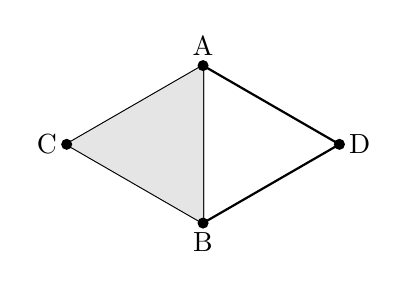
\begin{tikzpicture}[scale=1]
    \coordinate (A) at (0,1);
    \coordinate (B) at (0,-1);
    \coordinate (C) at (-1.7320508075688772,0); % -sqrt(3)
    \coordinate (D) at ( 1.7320508075688772,0); %  sqrt(3)

    % draw the two triangle perimeters (top--bottom is shared)
    \draw[thick] (C) -- (A) -- (B) -- cycle; % left triangle
    \draw[thick] (D) -- (A) -- (B) -- cycle; % right triangle

    \fill[gray!20] (C) -- (A) -- (B) -- cycle; % left triangle is solid

    % draw points and optional labels
    \foreach \p/\pos in {A/above,B/below,C/left,D/right}{
        \fill (\p) circle (2pt);
        \node[\pos] at (\p) {\p};
    }
\end{tikzpicture}
\end{center}
% \end{figure}

We will take an open cover indexed by the vertices, so $I=\bc{\mathrm{A,B,C,D}}$ in this case. For each point $\mathrm{P}\in I$, let ${U}_{\mathrm{P}}$ be the union of all simplices containing $\mathrm{P}$ minus the union of all simplices not containing $\mathrm{P}$. Therefore, for any $\sigma:[n]\to I$, $U_\sigma\neq\varnothing$ if and only if $\img(\sigma)$ is a simplex. An $n$-cochain is an assignment $f$ to each such $\sigma$ of an integer. Let $f$ be a closed $1$-form. It equivalently satisfies the following relations:
\begin{equation*}
\begin{array}{l@{}l@{\qquad}l}
    df(\mathrm{PPP}) = 0 & f(\mathrm{PP})=0, & \forall \mathrm{P}\in I, \\
    df(\mathrm{PQP}) = 0 \ \Leftrightarrow\ & f(\mathrm{PQ})=f(\mathrm{QP}), & \forall\bc{\mathrm{P,Q}}\neq\bc{\mathrm{C,D}}, \\
    df(\mathrm{ABC}) = 0 & \multicolumn{2}{@{}l}{f(\mathrm{BC})-f(\mathrm{AC})+f(\mathrm{AB})=0.}
\end{array}
\end{equation*}
But clearly, for $f$ to be a coboundary, we also need
\[
    f(\mathrm{AB}) + f(\mathrm{BD}) + f(\mathrm{DA}) = 0.
\]
This shows that $\cH^1(\mathcal{U},\Z)=\Z$, agreeing with the singular cohomology and the sheaf cohomology of $\Z$. Soon, we shall see that this is because $\mathcal{U}$ is a good cover.

\end{example}

Next, we decouple our definition of $\cC$ from the choice of the cover $\mathcal{U}$. This has an interesting side effect of effectively sheafifying $\mathcal{F}$ as well.

\begin{definition}
    Let $\mathcal{U,V}$ be open covers of $X$, indexed by $I,J$, respectively. A \emph{refinement map} is a set function $a:J\to I$ such that $V_{j}\subset U_{a(j)}$ for all $j\in J$. If a refinement map exists, we say $\mathcal{V}$ is a refinement of $\mathcal{U}$.
\end{definition}

A refinement map as above induces a morphism $\bar a:A_{\mathcal{U}}\to A_{\mathcal{V}}$ of cosimplicial objects by
\[
    \bar a(f)(\sigma) := f(a\circ\sigma),\quad \sigma:[n]\to J.
\]
Here we omitted a restriction map of $\mathcal{F}$ from $U_{a\circ\sigma}$ to $V_{\sigma}$.

Before taking the limit the category of open covers, whose morphisms are the refinement maps, is not filtered. To fix this, we need the following lemma.

\begin{lemma}
    If $a,b$ are both refinement maps $J\to I$, then the induced $\bar{a},\bar{b}$ are homotopic.
\end{lemma}

\begin{proof}
    The desired homotopy $\bar{a}\Rightarrow\bar{b}$ is a family of maps $h^{k,n}:A_{\mathcal{U}}^n \to A_{\mathcal{V}}^{n-1}$, $0\leq k\leq n-1$. For $\sigma:[n-1]\to J$ and $0\leq k\leq n-1$, put
    \[
        h^{k,n}(f)(\sigma) := f((b\circ\sigma_{\leq k})\cup (a\circ\sigma_{\geq k})).
    \]
    Again, the obvious restriction map is omitted. The notation should be self-explanatory.
    The conditions for $\{h^{k,n}\}$ to give a homotopy are the following: (the superscripts indicating $n$ is suppressed when appropriate)
    \begin{enumerate}[label=\arabic*), itemsep=3pt]
        \item $h^{0,n}\delta^0=\overline{a}^n$,\quad $h^{n-1,n}\delta^n=\overline{b}^n$,
        \item $h^{k}\delta^{i}=\delta^{i}h^{k+1}$,\quad if $i\leq k$,
        \item $h^{k}\delta^{i}=\delta^{i+1}h^{k}$,\quad if $i>k$,
        \item $h^{k}s^{j}=s^{j}h^{k-1}$,\quad if $j<k$,
        \item $h^{k}s^{j}=s^{j+1}h^{k}$,\quad if $j\geq k$.
    \end{enumerate}
    All of these follows immediately from the definitions.
\end{proof}

\begin{corollary}
    The cochain morphisms $\cC^{\bullet}(\mathcal{U},\mathcal{F})\to \cC^{\bullet}(\mathcal{V},\mathcal{F})$ induced by $a,b$ are homotopic. If $\mathcal{V}$ is a refinement of $\mathcal{U}$, then we have a well-defined $\cH^{\bullet}(\mathcal{U},\mathcal{F})\to \cH^{\bullet}(\mathcal{V},\mathcal{F})$.
\end{corollary}

\begin{proof}
    The (cosimplicial) Dold-Kan functor carries homotopic maps to homotopic maps, cf. \href{https://stacks.math.columbia.edu/tag/01A0}{stacks project}. Thus they induce the same map at cohomology level.
\end{proof}

\begin{corollary}
    For any presheaf $\mathcal{F}$, $\cH^{\bullet}(-,\mathcal{F})$ is a functor from the partial ordered set of open covers of $X$ to the category of graded abelian groups.
\end{corollary}

\begin{proof}
    Obvious.
\end{proof}

\begin{definition}
    The filtered colimit of the above functor is called the \emph{\Cech{} cohomology}, denoted by 
    \[
        \cH^{\bullet}(X,\mathcal{F}) := \varinjlim_{\mathcal{U}} \cH^{\bullet}(\mathcal{U},\mathcal{F}).
    \]
\end{definition}

\section{Example: Submanifold of \texorpdfstring{$\C$}{C}}

The first example of this theory is the Mittag-Leffler theorem in complex analysis.

Recall that a subset $A\subset X$ is \emph{relatively compact} if the closure of $A$ in $X$ is compact. 
\begin{lemma}\label{lem.holapprox}
    Let $U\subset\C$ be an open subset and let $L$ be a compact subset of $U$. Let $K$ be the union of $L$ with all components of $U\setminus L$ that are relatively compact in $U$. Then $K$ is compact, and any holomorphic function on $K$ can be uniformly approximated by holomorphic functions on $U$.
\end{lemma}

\begin{proof}
    If we can show that every bounded component of $\C\setminus K$ intersects $\C\setminus U$, then the result follows from Runge's approximation theorem, which we recall and prove below. To see this, suppose $C$ is a bounded component of $\C\setminus K$ fully contained in $U$. Then $\partial C\subset K\subset U$, so $C$ is relatively compact in $U$. We then see that $C$ is contained in a relatively compact component of $\C\setminus L$, a contradiction.
\end{proof}

\begin{theorem}[Runge]
    Let $K\subset\C$ be compact, and let $S\subset\C$ be that every bounded component of $\C\setminus K$ intersects $S$. Let $f$ be a holomorphic function on $K$. Then $f$ can be uniformly approximated by rational functions whose poles all lie in $S$.
\end{theorem}

For simplicity, we put
\[
    R_S := \bc{g\in\Gamma(K,\mathcal{O}):\exists\bc{R_n}\longrightarrow g\text{ uniformly on }K}
\]
where $R_n$ are rational functions with the only poles in $S$. It is easy to see that $R_S$ is a $\C$-algebra. This will be used in the proof.

The theorem now states that $R_S=\Gamma(K,\mathcal{O})$.

\begin{proof}
    Suppose $f\in\mathcal{O}(V)$ where $V$ is an open neighborhood of $K$. Take a compactly supported smooth $\psi$ such that $\psi\equiv 1$ on some neighborhood $W$ of $K$ and $\supp(\psi)\subset V$. Applying Lemma \ref{lem.cauchy} to $\psi f$ on an expanding sequence of bounded open sets containing $\supp(\psi)$, we obtain
    \[
        \psi f(a) - \frac{1}{2\pi i} \int_{\C} \frac{\partial\psi}{\partial\overline{z}} \frac{f(z)}{z-a} dz\wedge d\overline{z} =: h(a) \ \in \mathcal{O}(\C).
    \]
    By Cauchy's integral formula, $h$ is given by a power series. Therefore it has an obvious polynomial approximation by the partial sums which is clearly uniformly convergent on $K$. The task is then to approximate the integral
    \[
        g(a)
        := \int_{\C} \frac{\partial\psi}{\partial\overline{z}} \frac{f(z)}{z-a} dz\wedge d\overline{z}
        = \int_{V\setminus W} \frac{\partial\psi}{\partial\overline{z}} \frac{f(z)}{z-a} dz\wedge d\overline{z}.
    \]
    for $a\in W$. Note that the integrand is smooth in both $a$ and $z$. 
    
    Indeed, $g(a)$ can be uniformly approximated by constructing the Riemann sum
    \[
        \sum_{j} \frac{b_j}{z_j-a},\quad\text{finite sum}.
    \]
    where all $b_j\in\C$ and $z_j\notin K$. The only issue is that $z_j\notin S$ in general. Put
    \[
        Z = \bc{z\in\C\setminus K:(a-z)^{-1}\in R_S}.
    \]
    It remains to prove that $Z=\C\setminus K$.

    Suppose that $z\in Z$ and put $r=\dist(z,K)>0$. If $w\in B_r(z)$, then the series $\bc{Q_n}$ given by
    \[
        Q_n(a) := \sum_{k=0}^{n} \bp{\frac{w-z}{a-z}}^k \:\in\C[a][(a-z)^{-1}] \subset R_S
    \]
    is uniformly convergent on $K$ by the Weierstrass M-test, and converges to
    \[
        \bp{1-\frac{w-z}{a-z}}^{-1} = \frac{a-z}{a-w}.
    \]
    This shows that $(a-w)^{-1}\in R_S$, i.e., $w\in Z$. Thus $Z$ is open. Moreover, $\partial Z\subset K$ is clear, so $Z$ is also closed in $\C\setminus K$. It follows that every bounded component of $\C\setminus K$ is in $Z$.

    Finally, any $z$ with $\abs{z}\geq 2\sup_{a\in K}\abs{a}$ is in $Z$, so the unbounded component is also in $Z$.
\end{proof}

From this, we can deduce a global version of Lemma \ref{lem.cauchy}.
\begin{proposition}
    If $U$ is an open subset of $\C$ and $f\in\mathcal{A}\otimes\C(U)$, then there exists $g\in\mathcal{A}\otimes\C(U)$ such that $\dfrac{\partial}{\partial\overline{z}}g=f$.
\end{proposition}

\begin{proof}
    Pick a sequence $\bc{K_n}_n$ of compact sets such that $\bigcup K_n=U$, $K_n\subset\operatorname{int}(K_{n+1})$ and no component of $U\setminus K_n$ is relatively compact in $U$. Using Lemma \ref{lem.cauchy}, we get for each $n$ a function $g_n\in\mathcal{A}\otimes\C(U)$ such that $\dfrac{\partial}{\partial\overline{z}}g_n=f$ on some open neighborhood of $K_n$. It follows that $g_{n+1}-g_{n}$ is holomorphic on a neighborhood of $K_n$.

    With Lemma \ref{lem.holapprox}, let $u_n\in\mathcal{O}(U)$ such that $\abs{g_{n+1}-g_{n}-u_{n}}<2^{-n}$ on $K_n$. Put
    \[
        g := g_n + \sum_{m\geq n} \bp{g_{m+1}-g_{m}-u_{m}} - u_1 - u_2 - \cdots - u_{n-1},\quad\text{on }K_n.
    \]
    $g$ is obviously a well defined function on $U$. Morera's theorem implies that a uniform limit of holomorphic functions is holomorphic, so $g$ is the sum of $g_n$ and a holomorphic function on $K_n$. This completes the proof.
\end{proof}

\begin{theorem}[Mittag-Leffler]
    If $U$ is an open subset of $\C$ and $n\geq 1$, then $H^{n}(U,\mathcal{O})=0$.
\end{theorem}

\begin{remark}
    This result has a vast generalization known as Cartan's theorem B.
\end{remark}

\begin{proof}
    The above proposition shows that the complex of global sections of the Dolbeault complex is acyclic.
\end{proof}

\begin{corollary}
    Let $\mathcal{U}=\bc{U_i}_{i\in I}$ be a family of open subsets in $\C$ and $f_{ij}$ be holomorphic funtions on $U_i\cap U_j$ for all $i,j\in I$. If they satisy the cocycle condition
    \[
        f_{ij}+f_{jk}+f_{ki}=0
    \]
    for all $i,j,k\in I$, then there are holomorphic functions $f_i\in\mathcal{O}(U_i)$, such that $f_{ij}=f_i-f_j$.
\end{corollary}

\begin{proof}
    By Leray's theorem, $\cH^{1}(\mathcal{U},\mathcal{O})=H^{1}(U,\mathcal{O})=0$.
\end{proof}

\begin{definition}
    A \emph{meromorphic function} on a complex manifold $X$ is a holomorphic map $X\to\P^1$ that is not identically $\infty$. The sheaf of meromorphic functions will be denoted as $\mathcal{M}$.
\end{definition}

We have an exact sequence of $\mathcal{O}$-modules:
\[
    0 \longrightarrow \mathcal{O} \longrightarrow \mathcal{M} \xrightarrow{\ \pi\ } \mathcal{M}/\mathcal{O} \longrightarrow 0
\]
For each $x\in X$, the local map $\pi_x$ takes the \emph{principle part} of a meromorphic function at $x$.

\begin{theorem}
    Let $U$ be an open subset of $\C$ and $S$ be a discrete subset of $U$. Given, for each $x\in S$, a prescribed principle part
    \[
        (\mathcal{M}/\mathcal{O})_x \ni \mathfrak{p}_x := \sum_{n<0}b_n(z-x)^{-n},\text{ finite sum}.
    \]
    There exists a meromorphic function on $U$ whose poles are precisely given by the $\mathfrak{p}_x$.
\end{theorem}

\begin{proof}
    In the long exact sequence
    \[
        0 \longrightarrow H^0(U,\mathcal{O}) \longrightarrow H^0(U,\mathcal{M}) \xrightarrow{\ \pi^*\ } H^0(U,\mathcal{M}/\mathcal{O}) \longrightarrow H^1(U,\mathcal{O})
    \]
    By Mittag-Leffler's theorem, $H^1(U,\mathcal{O})=0$, so $\pi^*$ is a surjection.
\end{proof}

\begin{remark}
    We can obviously also prove this with the last corollary.
\end{remark}

\section*{The End}



\noindent Compiled on \todayymd.

\noindent\home

\end{document}

\documentclass{article}

\usepackage{geometry}
\usepackage{amsfonts, amsmath, amssymb, amsthm}
\usepackage{enumitem}
\usepackage{commands}
\usepackage{mathtools}
\usepackage{hyperref}
\usepackage{tikz}
\hypersetup{colorlinks, linkcolor={blue}, citecolor={blue}, urlcolor={blue}}

\newcommand{\dol}{\overline{\partial}}
\newcommand{\Cech}{\v{C}ech}
\newcommand{\cC}{\check{\mathcal{C}}}
\newcommand{\cH}{\check{\mathrm{H}}}

\begin{document}
\puttitle{What is Dolbeault cohomology}\self

\section{Preliminaries on complex manifolds}

A \emph{complex structure} $J$ on a real vector space $V$ is a linear map $J: V \to V$ such that $J^2 = -\id_V$. It equivalently provides a $\C$-vector space structure on $V$, so after complexification, we have a natural splitting
\[
    V \otimes_\R \C \simeq V_J \oplus \overline{V_J}
\]
into the two eigenspaces of $J\otimes \C$ with eigenvalues $\pm i$. 

An \emph{almost complex manifold} is a smooth manifold $M$ with a complex structure $J$ on the real tangent bundle $T$. The above discussion yields a splitting of complex vector bundles
\[
    T^*_{1,0}:=T^*,\quad T^*_{0,1}:=\overline{T^*},\quad T^* \otimes_\R \C \simeq T^*_{1,0} \oplus T^*_{0,1}.
\]
Since the exterior algebra functor $\Lambda^\bullet$ commutes with base change and colimits, we have
\[
    \Omega^i\otimes\C \simeq \Lambda^{i}(T^*\otimes\C) \simeq \bigoplus_{p+q=i} \Lambda^p(T^*_{1,0}) \otimes_\C \Lambda^q(T^*_{0,1}).
\]
To ease notation, denote the sheaves of $(p,q)$-forms by $\Omega^{p,q}\leftrightarrow \Lambda^p(T^*_{1,0}) \otimes \Lambda^q(T^*_{0,1})$. The (complexified) differential $d$ then decomposes as
\[
    d = \partial + \dol,
\]
where
\[
    \partial: \Omega^{p,q} \to \Omega^{p+1,q},\quad \dol: \Omega^{p,q} \to \Omega^{p,q+1}.
\]
These clearly satisfy $\partial^2 = 0$ and $\dol^2 = 0$, and hence also $\partial\dol+\dol\partial=0$.

In summary, the complexification of the de Rham complex $(\Omega^\bullet,d)$ results in a bigraded complex $(\Omega^{\bullet,\bullet},\partial,\dol)$.

\begin{definition}
    The \emph{Dolbeault complex} is the complex $(\Omega^{p,\bullet},\dol)$. The cohomology of the complex of its global sections is called the \emph{Dolbeault cohomology} and denoted by $H^{p,q}(M)$.
\end{definition}

So for example, if $p=0$, the Dolbeault complex is
\[
    0 \longrightarrow \Omega^{0,0} \xrightarrow{\ \dol\ } \Omega^{0,1} \xrightarrow{\ \dol\ } \Omega^{0,2} \longrightarrow \cdots
\]
and for higher $p$, the Dolbeault complex is obtained by tensoring the above with $\Omega^{p,0}$.

\begin{definition}
    A \emph{complex manifold} $(M,\mathcal{O})$ is a smooth manifold $(M,\mathcal{A})$ with a sheaf of holomorphic functions $\mathcal{O}\subset\mathcal{A}\otimes\C$, such that $\mathcal{O}$ is locally isomorphic to the sheaf of holomorphic functions on open subsets of $\C^n$.
\end{definition}

In this case, $T_{1,0}\simeq T$, as a $\C$-vector bundle, has a natural holomorphic structure. Hence it is sometimes called the \emph{holomorphic tangent bundle}.

Finally, consider the following analogue of the de Rham complex
\begin{equation}\label{eq:dol}
    0 \longrightarrow \mathcal{O} \longrightarrow \mathcal{A}\otimes\C \xrightarrow{\ \dol\ } \Omega^{0,1} \xrightarrow{\ \dol\ } \Omega^{0,2} \longrightarrow \cdots
\end{equation}
All the sheaves $\Omega^{\bullet,\bullet}$ are soft as $\mathcal{A}$-modules. To compute the cohomology, we have 

\begin{theorem}\label{thm.poin}
    \eqref{eq:dol} is exact, so the Dolbeault complex is a soft resolution of $\mathcal{O}$.
\end{theorem}

We defer the proof of this to the next section. 

\begin{corollary}
    Given any holomorphic vector bundle $E$, the following sequence is a soft resolution for the corresponding locally free $\mathcal{O}$-module $\mathcal{E}$.
    \[
        0 \longrightarrow \mathcal{E} \longrightarrow (\mathcal{A}\otimes\C)\otimes\mathcal{E} \xrightarrow{\ \dol\ } \Omega^{0,1}\otimes\mathcal{E} \xrightarrow{\ \dol\ } \, \cdots\, \xrightarrow{\ \dol\ } \Omega^{0,n}\otimes\mathcal{E} \longrightarrow 0
    \]
\end{corollary}

\begin{proof}
    Since $\dol$ is $\mathcal{O}$-linear, we apply $-\otimes_{\mathcal{O}}\mathcal{E}$ to \eqref{eq:dol}.
\end{proof}

Define $\mathcal{E}':=(\mathcal{A}\otimes\C)\otimes_{\mathcal{O}}\mathcal{E}$ if we wish to consider the sheaf of smooth sections instead. Any toddler will know how to rewrite the above resolution as
\[
    0 \longrightarrow \mathcal{E} \longrightarrow \mathcal{E}' \xrightarrow{\ \dol\ } \Omega^{0,1}\otimes\mathcal{E}' \xrightarrow{\ \dol\ } \, \cdots\, \xrightarrow{\ \dol\ } \Omega^{0,n}\otimes\mathcal{E}' \longrightarrow 0
\]
where $\otimes=\otimes_{\mathcal{A}\otimes\C}$. In particular, we've explained previously that the vector bundles corresponding to $\Omega^{p,0}$ are in fact holomorphic vector bundles. We quickly deduce that
\[
    0 \longrightarrow \mathcal{H}^p \longrightarrow \Omega^{p,0} \xrightarrow{\ \dol\ } \Omega^{p,1} \xrightarrow{\ \dol\ } \, \cdots\, \xrightarrow{\ \dol\ } \Omega^{p,n} \longrightarrow 0
\]
is a soft resolution for $\mathcal{H}^p$, the sheaf of holomorphic $p$-forms. Therefore

\begin{corollary}
    The Dolbeault cohomology with coefficients in a holomorphic vector bundle $E$ satisfies
    \[
        H^{p,q}(M,E) \simeq H^q(M,\mathcal{E}\otimes\mathcal{H}^p).
    \]
    In particular, $H^{p,q}(M) \simeq H^q(M,\mathcal{H}^p)$, and so $H^{0,q}(M) \simeq H^q(M,\mathcal{O})$.
\end{corollary}

\section{Dolbeault-Grothendieck Lemma}

In the results of this section, we will take smooth sections defined globally on some affine space $\C^n$ and discuss their properties over a certain open subset $V$. However, it clearly suffices to define these functions on any neighborhood of $\overline{V}$.

\begin{lemma}\label{lem.cauchy}
    If $V$ is a bounded open subset of $\C$ and $f\in\mathcal{A}\otimes\C(\C)$ is compactly supported, then there exists $g\in\mathcal{A}\otimes\C(\C)$ such that $\dfrac{\partial}{\partial\overline{z}}g=f$ on $V$. One such $g$ is given by the formula
    \[
        g(a) := \frac{1}{2\pi i} \int_{V} \frac{f(z)}{z-a} dz\wedge d\overline{z},\quad \forall a\in\C.
    \]
\end{lemma}

\begin{proof}
    First, let's check that this integral makes sense. For small $\epsilon>0$, put $W=B_\epsilon(a)$. Since $dz\wedge d\overline{z}=-2i d\lambda=-2i\rho d\rho\wedge d\theta$, where $\lambda$ is the usual Lebesgue measure, we have
    \begin{align*}
        \int_{W} \abs{\frac{f(z)}{z-a}} d\lambda 
        = \int_{[0,2\pi]\times[0,\varepsilon]} \abs{\frac{f(a+\rho e^{i\theta})}{\rho e^{i\theta}}} \rho d\rho d\theta 
        = \int \abs{f(a+\rho e^{i\theta})} d\rho d\theta
        < \infty,
    \end{align*}
    where the first equality is the change of variable formula for non-negative functions, cf. \emph{Folland, Theorem 2.47}. Away from $W$, the integrand is smooth. This shows that $g$ is well defined. 
    
    If the singularity at $a$ is in $V$, one way to deal with it is the following trick. Take a smooth function $\mu$ such that $\mu(W)=1$ and $\supp(\mu)\subset V$. Consider
    \begin{align*}
        g_1(a) 
        &:= \int_{V}\frac{(\mu f)(z)}{z-a}dz\wedge d\overline{z} \\
        &= \int_{\C}\frac{(\mu f)(z)}{z-a}dz\wedge d\overline{z} \\
        &= \int_{\C\setminus\bc{0}}\frac{(\mu f)(w+a)}{w}dw\wedge d\overline{w}
    \end{align*}
    where the substitution $w=z-a$ is used. For the same reason as above, the function
    \[
        \frac{\partial}{\partial\overline{a}}\frac{(\mu f)(w+a)}{w}
        = \frac{1}{w}\frac{\partial}{\partial\overline{a}}(\mu f)(w+a)
    \]
    is Lebesgue integrable, so the \href{https://en.wikipedia.org/wiki/Leibniz_integral_rule#Measure_theory_statement}{Leibniz integral rule} applies. Furthermore, notice that
    \[
        \frac{1}{w}\frac{\partial}{\partial\overline{a}}(\mu f)(w+a)
        = \frac{1}{w}\frac{\partial}{\partial\overline{w}}(\mu f)(w+a)
        = \frac{\partial}{\partial\overline{w}}\frac{(\mu f)(w+a)}{w},
    \]
    as $1/w$ is holomorphic on the punctured plane. We thus have
    \begin{align*}
        \frac{\partial}{\partial\overline{a}}g_1(a)
        &= \int_{\C\setminus\bc{0}} \frac{\partial}{\partial\overline{w}}\frac{(\mu f)(w+a)}{w} dw\wedge d\overline{w} \\
        &= -\lim_{\varepsilon\to 0} \int_{B_{514}(0)\setminus B_{\varepsilon}(0)} d\bp{\frac{(\mu f)(w+a)}{w} dw} \\
        &= \lim_{\varepsilon\to 0} \int_{\abs{w}=\varepsilon} \frac{(\mu f)(w+a)}{w} dw \quad(\because\text{Stokes' formula})\\
        &= \lim_{\varepsilon\to 0} \int_{0}^{2\pi} \frac{(\mu f)(\varepsilon e^{i\theta}+a)}{\varepsilon e^{i\theta}} \frac{d\bp{\varepsilon e^{i\theta}}}{d\theta}d\theta \\
        &= 2\pi i f(a).
    \end{align*}

    It remains to show that $\dfrac{\partial}{\partial\overline{a}}g_2(a)=0$, where
    \begin{align*}
        g_2(a) 
        &:= \int_{V}\frac{\bp{(1-\mu)f}(z)}{z-a}dz\wedge d\overline{z} \\
        &= \int_{V\setminus W}\frac{\bp{(1-\mu)f}(z)}{z-a}dz\wedge d\overline{z}.
    \end{align*}
    This is obvious, since $1/(z-a)$ is holomorphic away from $W$; the Leibniz rule automatically applies. We have $g=(g_1+g_2)/(2\pi i)$, and the proof is complete.
\end{proof}

Denote $D_r:=B_r(0)$.

\begin{proposition}[Dolbeault-Grothendieck Lemma, local version]
    Fix $n>0$, $r>0$, and let $V=D_r^n$. Given $\omega\in\Omega^{p,q}(\C^n)$ with $q>0$, if $\dol\omega=0$, then there exists $\xi\in\Omega^{p,q-1}(\C^n)$ such that $\omega=\dol\xi$ on $V$.
\end{proposition}

\begin{proof}
    WLOG assume $p=0$. We will induct on $n$. But first, we need to strengthen the statement to let $\omega$ and $\xi$ depend holomorphically on a parameter $t\in D^m$, where $m$ and the radii are arbitrary. When we use $\dol$, we view $t$ as fixed and never take its differential. We emphasize this by changing the notation to
    \[
        \dol_n \xi(t) \overset{!}{=} \omega(t).
    \]

    The base case $n=1$ is handled by the above lemma. $\xi$, given by an explicit integral, depends holomorphically on $t$.
    
    Let $n\geq 2$ and assume the result for $n-1$. Denote the holomorphic coordinates as $z_1,\cdots,z_n$. We have a unique decomposition
    \[
        \omega(t) =: \omega_1(t,z_n) \wedge d\overline{z_n} + \omega_2(t,z_n)
    \]
    where $\omega_1$, $\omega_2$ does not contain the form $d\overline{z_n}$. Hence they are forms on $n-1$ complex variables and $m+1$ parameters ($(t,z_n)\in D^{m+1}$). We have
    \[
        0 = \dol_n\omega(t) = \bp{\dol_{n-1}\omega_1(t,z_n)+(-1)^q\frac{\partial}{\partial\overline{z_n}}\omega_2(t,z_n)}\wedge d\overline{z_n} + \dol_{n-1}\omega_2(t,z_n).
    \]
    Hence
    \begin{gather}
        \dol_{n-1}\omega_2(t,z_n) = 0 \label{eq.1}\\
        \dol_{n-1}\omega_1(t,z_n)+(-1)^q\frac{\partial}{\partial\overline{z_n}}\omega_2(t,z_n) = 0 \label{eq.2}
    \end{gather}

    Take $r'>r$ and put $V_{1}=D_{r}^{n-1}$, $V_{1}'=D_{r'}^{n-1}$. By using the induction hypothesis on \eqref{eq.1}, we obtain a form $\alpha(t,z_n)$ such that $\dol_{n-1}\alpha=\omega_2$ on $V_{1}'$. Notice that
    \[
        \frac{\partial}{\partial\overline{z_n}}\omega_2
        = \frac{\partial}{\partial\overline{z_n}}\dol_{n-1}\alpha
        = \dol_{n-1}\frac{\partial}{\partial\overline{z_n}}\alpha.
    \]
    Plugging this into \eqref{eq.2}, we get another form $\beta(t,z_n)$, satisfying on $V_{1}$
    \[
        \dol_{n-1}\beta 
        = \omega_1 + (-1)^q \frac{\partial}{\partial\overline{z_n}}\alpha. 
    \]

    We can now put
    \[
        \xi_1 := \beta,\quad \xi_2 := \alpha,\quad \xi:=\xi_1\wedge d\overline{z_n} + \xi_2.
    \]
    It is clear that $\dol_n\xi=\omega$ on $V$, and the proof is complete.
\end{proof}

\begin{proof}[Proof of Theorem \ref{thm.poin}]
    The exactness at the first three terms
    \[
        0 \longrightarrow \mathcal{O} \longrightarrow \mathcal{A}\otimes\C \xrightarrow{\ \dol\ } \Omega^{0,1}
    \]
    is trivial. Let $n=\dim_\C(M)$. Fix $q\in\Z_{>0}$, a point in $M$ and a neighborhood $U$ biholomorphic to a polydisk $D^n\subset\C^n$. For all $\omega\in\Omega^{0,q}(U)$ satisfying $\dol\omega=0$, the above proposition yields $\xi\in\Omega^{0,q-1}(U)$ such that $\dol\xi=\omega$ holds locally.
\end{proof}

\begin{remark}
    This proof is essentially the same as the de Rham theorem, where instead of the lemma, we simply use the Fundamental Theorem of Calculus there. 
\end{remark}

\section{\Cech{} cohomology}

The \Cech{} method is a way to directly compute sheaf cohomology.

Fix an open cover $\mathcal{U}=\bc{U_i:i\in I}$ of a space $X$. The associated \emph{\Cech{} nerve} is the simplicial set whose $n$-th simplices are set functions $\sigma:[n]\to I$ such that 
\[
    U_{\sigma}:=U_{\sigma_{0}}\cap U_{\sigma_{1}}\cap\cdots\cap U_{\sigma_{n}}\neq\varnothing.
\]
(This condition is not crucial here, but is devised for purposes such as the nerve theorem.) Given a presheaf $\mathcal{F}$ of abelian groups, we define a \emph{co-}simplicial abelian group $A$, with the group of $n$-simplicies given by
\[
    A^n := \prod_{\sigma:[n]\to I}\mathcal{F}(U_\sigma).
\]
In other words, an $n$-cochain is an assignment to each 'geometric $n$-simplex' $\sigma$ of an element of $\mathcal{F}(U_\sigma)$. The co-degeneracy maps $s^j:A^{n}\to A^{n-1}$ are evident, induced by the identity map of the group of sections over $U_{\sigma}=U_{\sigma\circ s^j}$. The co-face maps $\delta^i:A^{n}\to A^{n+1}$ are defined component-wise by the composition
\[
    A^{n} \xrightarrow{\text{proj}} \mathcal{F}(U_{\sigma\circ\delta^i}) \longrightarrow \mathcal{F}(U_{\sigma}),
    \quad \sigma\in I^{[n+1]},
\]
where the second morphism is the restriction.

Under the Dold-Kan correspondence, we then have the following notion of cohomology.
\begin{definition}
    The Moore cochain complex given by $A$ is called the \emph{\Cech{} complex} of $\mathcal{F}$ with respect to the cover $\mathcal{U}$, denoted by $\cC^{\bullet}(\mathcal{U},\mathcal{F})$. Its cohomology is denoted by $\cH^\bullet(\mathcal{U},\mathcal{F})$.
\end{definition}

By definition, $\cC^{n}(\mathcal{U},\mathcal{F})=A^n$, and $d^n:A^{n}\to A^{n+1}$ is given by $d^n = \sum_{i=0}^{n+1} (-1)^i\delta^i$.

\begin{example}

Let's see a dumb example that may be helpful. Consider a geometrically realized finite simplicial complex, say this one below. Let $\mathcal{F}$ be the constant sheaf $\Z$.

% \begin{figure}[htb!]
\begin{center}
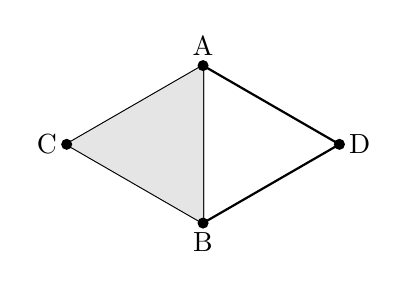
\begin{tikzpicture}[scale=1]
    \coordinate (A) at (0,1);
    \coordinate (B) at (0,-1);
    \coordinate (C) at (-1.7320508075688772,0); % -sqrt(3)
    \coordinate (D) at ( 1.7320508075688772,0); %  sqrt(3)

    % draw the two triangle perimeters (top--bottom is shared)
    \draw[thick] (C) -- (A) -- (B) -- cycle; % left triangle
    \draw[thick] (D) -- (A) -- (B) -- cycle; % right triangle

    \fill[gray!20] (C) -- (A) -- (B) -- cycle; % left triangle is solid

    % draw points and optional labels
    \foreach \p/\pos in {A/above,B/below,C/left,D/right}{
        \fill (\p) circle (2pt);
        \node[\pos] at (\p) {\p};
    }
\end{tikzpicture}
\end{center}
% \end{figure}

We will take an open cover indexed by the vertices, so $I=\bc{\mathrm{A,B,C,D}}$ in this case. For each point $\mathrm{P}\in I$, let ${U}_{\mathrm{P}}$ be the union of all simplices containing $\mathrm{P}$ minus the union of all simplices not containing $\mathrm{P}$. Therefore, for any $\sigma:[n]\to I$, $U_\sigma\neq\varnothing$ if and only if $\img(\sigma)$ is a simplex. An $n$-cochain is an assignment $f$ to each such $\sigma$ of an integer. Let $f$ be a closed $1$-form. It equivalently satisfies the following relations:
\begin{equation*}
\begin{array}{l@{}l@{\qquad}l}
    df(\mathrm{PPP}) = 0 & f(\mathrm{PP})=0, & \forall \mathrm{P}\in I, \\
    df(\mathrm{PQP}) = 0 \ \Leftrightarrow\ & f(\mathrm{PQ})=f(\mathrm{QP}), & \forall\bc{\mathrm{P,Q}}\neq\bc{\mathrm{C,D}}, \\
    df(\mathrm{ABC}) = 0 & \multicolumn{2}{@{}l}{f(\mathrm{BC})-f(\mathrm{AC})+f(\mathrm{AB})=0.}
\end{array}
\end{equation*}
But clearly, for $f$ to be a coboundary, we also need
\[
    f(\mathrm{AB}) + f(\mathrm{BD}) + f(\mathrm{DA}) = 0.
\]
This shows that $\cH^1(\mathcal{U},\Z)=\Z$, agreeing with the singular cohomology and the sheaf cohomology of $\Z$. Soon, we shall see that this is because $\mathcal{U}$ is a good cover.

\end{example}

Next, we decouple our definition of $\cC$ from the choice of the cover $\mathcal{U}$. This has an interesting side effect of effectively sheafifying $\mathcal{F}$ as well.

\begin{definition}
    Let $\mathcal{U,V}$ be open covers of $X$, indexed by $I,J$, respectively. A \emph{refinement map} is a set function $a:J\to I$ such that $V_{j}\subset U_{a(j)}$ for all $j\in J$. If a refinement map exists, we say $\mathcal{V}$ is a refinement of $\mathcal{U}$.
\end{definition}

A refinement map as above induces a morphism $\bar a:A_{\mathcal{U}}\to A_{\mathcal{V}}$ of cosimplicial objects by
\[
    \bar a(f)(\sigma) := f(a\circ\sigma),\quad \sigma:[n]\to J.
\]
Here we omitted a restriction map of $\mathcal{F}$ from $U_{a\circ\sigma}$ to $V_{\sigma}$.

Before taking the limit the category of open covers, whose morphisms are the refinement maps, is not filtered. To fix this, we need the following lemma.

\begin{lemma}
    If $a,b$ are both refinement maps $J\to I$, then the induced $\bar{a},\bar{b}$ are homotopic.
\end{lemma}

\begin{proof}
    The desired homotopy $\bar{a}\Rightarrow\bar{b}$ is a family of maps $h^{k,n}:A_{\mathcal{U}}^n \to A_{\mathcal{V}}^{n-1}$, $0\leq k\leq n-1$. For $\sigma:[n-1]\to J$ and $0\leq k\leq n-1$, put
    \[
        h^{k,n}(f)(\sigma) := f((b\circ\sigma_{\leq k})\cup (a\circ\sigma_{\geq k})).
    \]
    Again, the obvious restriction map is omitted. The notation should be self-explanatory.
    The conditions for $\{h^{k,n}\}$ to give a homotopy are the following: (the superscripts indicating $n$ is suppressed when appropriate)
    \begin{enumerate}[label=\arabic*), itemsep=3pt]
        \item $h^{0,n}\delta^0=\overline{a}^n$,\quad $h^{n-1,n}\delta^n=\overline{b}^n$,
        \item $h^{k}\delta^{i}=\delta^{i}h^{k+1}$,\quad if $i\leq k$,
        \item $h^{k}\delta^{i}=\delta^{i+1}h^{k}$,\quad if $i>k$,
        \item $h^{k}s^{j}=s^{j}h^{k-1}$,\quad if $j<k$,
        \item $h^{k}s^{j}=s^{j+1}h^{k}$,\quad if $j\geq k$.
    \end{enumerate}
    All of these follows immediately from the definitions.
\end{proof}

\begin{corollary}
    The cochain morphisms $\cC^{\bullet}(\mathcal{U},\mathcal{F})\to \cC^{\bullet}(\mathcal{V},\mathcal{F})$ induced by $a,b$ are homotopic. If $\mathcal{V}$ is a refinement of $\mathcal{U}$, then we have a well-defined $\cH^{\bullet}(\mathcal{U},\mathcal{F})\to \cH^{\bullet}(\mathcal{V},\mathcal{F})$.
\end{corollary}

\begin{proof}
    The (cosimplicial) Dold-Kan functor carries homotopic maps to homotopic maps, cf. \href{https://stacks.math.columbia.edu/tag/01A0}{stacks project}. Thus they induce the same map at cohomology level.
\end{proof}

\begin{corollary}
    For any presheaf $\mathcal{F}$, $\cH^{\bullet}(-,\mathcal{F})$ is a functor from the partial ordered set of open covers of $X$ to the category of graded abelian groups.
\end{corollary}

\begin{proof}
    Obvious.
\end{proof}

\begin{definition}
    The filtered colimit of the above functor is called the \emph{\Cech{} cohomology}, denoted by 
    \[
        \cH^{\bullet}(X,\mathcal{F}) := \varinjlim_{\mathcal{U}} \cH^{\bullet}(\mathcal{U},\mathcal{F}).
    \]
\end{definition}

\section{Example: Submanifold of \texorpdfstring{$\C$}{C}}

The first example of this theory is the Mittag-Leffler theorem in complex analysis.

Recall that a subset $A\subset X$ is \emph{relatively compact} if the closure of $A$ in $X$ is compact. 
\begin{lemma}\label{lem.holapprox}
    Let $U\subset\C$ be an open subset and let $L$ be a compact subset of $U$. Let $K$ be the union of $L$ with all components of $U\setminus L$ that are relatively compact in $U$. Then $K$ is compact, and any holomorphic function on $K$ can be uniformly approximated by holomorphic functions on $U$.
\end{lemma}

\begin{proof}
    If we can show that every bounded component of $\C\setminus K$ intersects $\C\setminus U$, then the result follows from Runge's approximation theorem, which we recall and prove below. To see this, suppose $C$ is a bounded component of $\C\setminus K$ fully contained in $U$. Then $\partial C\subset K\subset U$, so $C$ is relatively compact in $U$. We then see that $C$ is contained in a relatively compact component of $\C\setminus L$, a contradiction.
\end{proof}

\begin{theorem}[Runge]
    Let $K\subset\C$ be compact, and let $S\subset\C$ be that every bounded component of $\C\setminus K$ intersects $S$. Let $f$ be a holomorphic function on $K$. Then $f$ can be uniformly approximated by rational functions whose poles all lie in $S$.
\end{theorem}

For simplicity, we put
\[
    R_S := \bc{g\in\Gamma(K,\mathcal{O}):\exists\bc{R_n}\longrightarrow g\text{ uniformly on }K}
\]
where $R_n$ are rational functions with the only poles in $S$. It is easy to see that $R_S$ is a $\C$-algebra. This will be used in the proof.

The theorem now states that $R_S=\Gamma(K,\mathcal{O})$.

\begin{proof}
    Suppose $f\in\mathcal{O}(V)$ where $V$ is an open neighborhood of $K$. Take a compactly supported smooth $\psi$ such that $\psi\equiv 1$ on some neighborhood $W$ of $K$ and $\supp(\psi)\subset V$. Applying Lemma \ref{lem.cauchy} to $\psi f$ on an expanding sequence of bounded open sets containing $\supp(\psi)$, we obtain
    \[
        \psi f(a) - \frac{1}{2\pi i} \int_{\C} \frac{\partial\psi}{\partial\overline{z}} \frac{f(z)}{z-a} dz\wedge d\overline{z} =: h(a) \ \in \mathcal{O}(\C).
    \]
    By Cauchy's integral formula, $h$ is given by a power series. Therefore it has an obvious polynomial approximation by the partial sums which is clearly uniformly convergent on $K$. The task is then to approximate the integral
    \[
        g(a)
        := \int_{\C} \frac{\partial\psi}{\partial\overline{z}} \frac{f(z)}{z-a} dz\wedge d\overline{z}
        = \int_{V\setminus W} \frac{\partial\psi}{\partial\overline{z}} \frac{f(z)}{z-a} dz\wedge d\overline{z}.
    \]
    for $a\in W$. Note that the integrand is smooth in both $a$ and $z$. 
    
    Indeed, $g(a)$ can be uniformly approximated by constructing the Riemann sum
    \[
        \sum_{j} \frac{b_j}{z_j-a},\quad\text{finite sum}.
    \]
    where all $b_j\in\C$ and $z_j\notin K$. The only issue is that $z_j\notin S$ in general. Put
    \[
        Z = \bc{z\in\C\setminus K:(a-z)^{-1}\in R_S}.
    \]
    It remains to prove that $Z=\C\setminus K$.

    Suppose that $z\in Z$ and put $r=\dist(z,K)>0$. If $w\in B_r(z)$, then the series $\bc{Q_n}$ given by
    \[
        Q_n(a) := \sum_{k=0}^{n} \bp{\frac{w-z}{a-z}}^k \:\in\C[a][(a-z)^{-1}] \subset R_S
    \]
    is uniformly convergent on $K$ by the Weierstrass M-test, and converges to
    \[
        \bp{1-\frac{w-z}{a-z}}^{-1} = \frac{a-z}{a-w}.
    \]
    This shows that $(a-w)^{-1}\in R_S$, i.e., $w\in Z$. Thus $Z$ is open. Moreover, $\partial Z\subset K$ is clear, so $Z$ is also closed in $\C\setminus K$. It follows that every bounded component of $\C\setminus K$ is in $Z$.

    Finally, any $z$ with $\abs{z}\geq 2\sup_{a\in K}\abs{a}$ is in $Z$, so the unbounded component is also in $Z$.
\end{proof}

From this, we can deduce a global version of Lemma \ref{lem.cauchy}.
\begin{proposition}
    If $U$ is an open subset of $\C$ and $f\in\mathcal{A}\otimes\C(U)$, then there exists $g\in\mathcal{A}\otimes\C(U)$ such that $\dfrac{\partial}{\partial\overline{z}}g=f$.
\end{proposition}

\begin{proof}
    Pick a sequence $\bc{K_n}_n$ of compact sets such that $\bigcup K_n=U$, $K_n\subset\operatorname{int}(K_{n+1})$ and no component of $U\setminus K_n$ is relatively compact in $U$. Using Lemma \ref{lem.cauchy}, we get for each $n$ a function $g_n\in\mathcal{A}\otimes\C(U)$ such that $\dfrac{\partial}{\partial\overline{z}}g_n=f$ on some open neighborhood of $K_n$. It follows that $g_{n+1}-g_{n}$ is holomorphic on a neighborhood of $K_n$.

    With Lemma \ref{lem.holapprox}, let $u_n\in\mathcal{O}(U)$ such that $\abs{g_{n+1}-g_{n}-u_{n}}<2^{-n}$ on $K_n$. Put
    \[
        g := g_n + \sum_{m\geq n} \bp{g_{m+1}-g_{m}-u_{m}} - u_1 - u_2 - \cdots - u_{n-1},\quad\text{on }K_n.
    \]
    $g$ is obviously a well defined function on $U$. Morera's theorem implies that a uniform limit of holomorphic functions is holomorphic, so $g$ is the sum of $g_n$ and a holomorphic function on $K_n$. This completes the proof.
\end{proof}

\begin{theorem}[Mittag-Leffler]
    If $U$ is an open subset of $\C$ and $n\geq 1$, then $H^{n}(U,\mathcal{O})=0$.
\end{theorem}

\begin{remark}
    This result has a vast generalization known as Cartan's theorem B.
\end{remark}

\begin{proof}
    The above proposition shows that the complex of global sections of the Dolbeault complex is acyclic.
\end{proof}

\begin{corollary}
    Let $\mathcal{U}=\bc{U_i}_{i\in I}$ be a family of open subsets in $\C$ and $f_{ij}$ be holomorphic funtions on $U_i\cap U_j$ for all $i,j\in I$. If they satisy the cocycle condition
    \[
        f_{ij}+f_{jk}+f_{ki}=0
    \]
    for all $i,j,k\in I$, then there are holomorphic functions $f_i\in\mathcal{O}(U_i)$, such that $f_{ij}=f_i-f_j$.
\end{corollary}

\begin{proof}
    By Leray's theorem, $\cH^{1}(\mathcal{U},\mathcal{O})=H^{1}(U,\mathcal{O})=0$.
\end{proof}

\begin{definition}
    A \emph{meromorphic function} on a complex manifold $X$ is a holomorphic map $X\to\P^1$ that is not identically $\infty$. The sheaf of meromorphic functions will be denoted as $\mathcal{M}$.
\end{definition}

We have an exact sequence of $\mathcal{O}$-modules:
\[
    0 \longrightarrow \mathcal{O} \longrightarrow \mathcal{M} \xrightarrow{\ \pi\ } \mathcal{M}/\mathcal{O} \longrightarrow 0
\]
For each $x\in X$, the local map $\pi_x$ takes the \emph{principle part} of a meromorphic function at $x$.

\begin{theorem}
    Let $U$ be an open subset of $\C$ and $S$ be a discrete subset of $U$. Given, for each $x\in S$, a prescribed principle part
    \[
        (\mathcal{M}/\mathcal{O})_x \ni \mathfrak{p}_x := \sum_{n<0}b_n(z-x)^{-n},\text{ finite sum}.
    \]
    There exists a meromorphic function on $U$ whose poles are precisely given by the $\mathfrak{p}_x$.
\end{theorem}

\begin{proof}
    In the long exact sequence
    \[
        0 \longrightarrow H^0(U,\mathcal{O}) \longrightarrow H^0(U,\mathcal{M}) \xrightarrow{\ \pi^*\ } H^0(U,\mathcal{M}/\mathcal{O}) \longrightarrow H^1(U,\mathcal{O})
    \]
    By Mittag-Leffler's theorem, $H^1(U,\mathcal{O})=0$, so $\pi^*$ is a surjection.
\end{proof}

\begin{remark}
    We can obviously also prove this with the last corollary. Test
\end{remark}

\section{Computations}

The standard example of Dolbeault cohomology is the complex projective space $\P^n$.

\section*{The End}



\noindent Compiled on \todayymd.

\noindent\home

\end{document}
